%!TEX root = ../template.tex
%%%%%%%%%%%%%%%%%%%%%%%%%%%%%%%%%%%%%%%%%%%%%%%%%%%%%%%%%%%%%%%%%%%%
%% chapter4.tex
%% NOVA thesis document file
%%
%% Chapter with lots of dummy text
%%%%%%%%%%%%%%%%%%%%%%%%%%%%%%%%%%%%%%%%%%%%%%%%%%%%%%%%%%%%%%%%%%%%
\chapter{Implementation prototype}
\label{cha:workplan}

TODO - falar daquilo de como sabemos se as cenas estão mesmo a correr na enclave (e apontar po site do scone onde mostram o programa que ve isso)

\section{Architecture and implemented components}



Rebobinar o boneco da arquitetura
Dizer que tecnologias são responsaveis por o que. ex: redis 6.0.2 é a KVS, Cloud OVH, o Intel Modelo X é o processador, oferece X Mbs de page cache, tem esta RAM, etc etc...

\section{Implementation options}
\subsection{TEE-REDIS solution}
Descrever a solucao com detalhes de tecnologias
\subsection{Client-based benchmarks}


Experimental evaluation of the prototype, to study the overheads of TREDIS against a no trusted REDIS solution. For this purpose we will analyze: (1) Performance conditions observed by latency and throughput measurements; (2) Adequacy to manage operations on privacy-enhanced big-datasets; (3) Scalability conditions under different client-workloads; (4) Analysis of required resources, including memory, CPU, I/O and energy.
\section{Tradeoffs on the implementation options}
Discutir overheads daquilo que usámos (openSSL issue, redis monolitico ou não, etc)
\section{Summary}


In this chapter, we present our work plan for the elaboration phase of the dissertation. The plan is represented in figure \ref{fig:ganttPlannedTasks}. This plan was designed to meet the calendar of the second semester in FCT-UNL, while also taking into account personal vacation dates. As represented in the plan, the main activities related to developments and experimental evaluations of prototypes will be conducted until the second week of August. 
We consider to write a paper as an open possibility, to be submitted to a specialized workshop in the dissertation topic. Depending on the evolution of the implementation and experimental evaluation tasks we can consider a submission to Inforum 2020 or to another target.

The remaining time until the middle of September 2020 will be dedicated to final implementation refinements and final experimental evaluations on a cloud-provided solution, provided "as a service". The effort of the report-writing activities will be balanced and developed in different cycles in the period from the middle of April 2020 to the first week of September 2020. We planned the second and third week of September for the final revision of the dissertation report, before the submission to the jury. 

The tasks represented in the plan are described in more detail in the table represented in figure \ref{fig:taskDescription}. In this table, tasks are presented with a little more insight, while also referring the relevant dependencies.

\newpage

\begin{figure}[htbp]
	\centerline{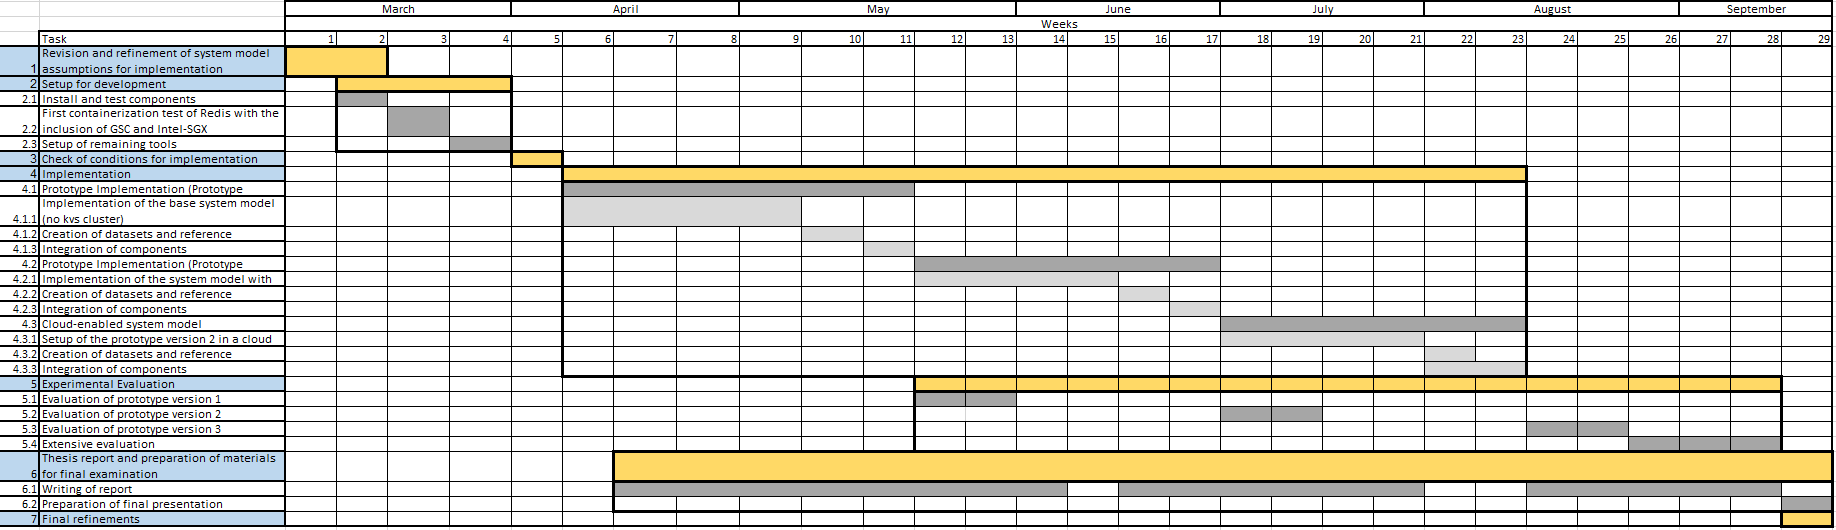
\includegraphics[angle=90, width=0.448\linewidth]{ganttchap4}}
	\caption{Detailed tasks}
	\label{fig:ganttPlannedTasks}
\end{figure}

\newpage

\begin{figure}[htbp]
	\centerline{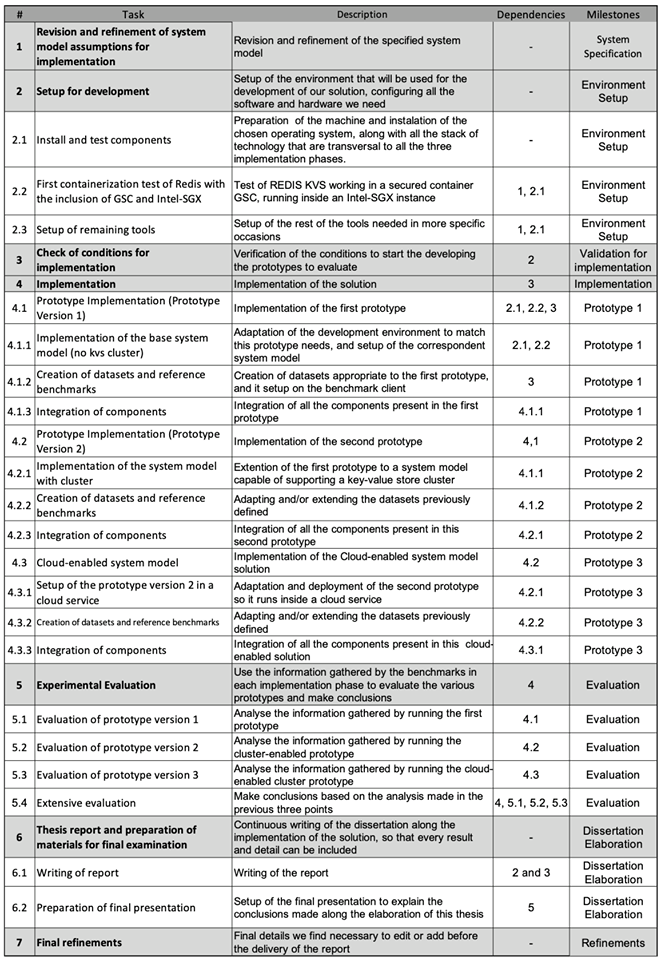
\includegraphics[angle=0, width=0.88\linewidth]{taskDescriptionv2}}
	\caption{Description of tasks}
	\label{fig:taskDescription}
\end{figure}


% \lipsum[1-100]
% \lipsum[1-700]
% \lipsum[1-700]
% \lipsum[1-700]
% \lipsum[1-700]
% \lipsum[1-700]
% \lipsum[1-700]
% \lipsum[1-700]
% \lipsum[1-700]
